\documentclass[aspectratio=169]{beamer}
\usepackage[utf8]{inputenc}\usepackage[T1]{fontenc}\usepackage{lmodern}
\usetheme{Madrid}
\setbeamertemplate{navigation symbols}{}
\setbeamercovered{transparent}
\setbeamertemplate{itemize items}[circle]
\setbeamertemplate{enumerate items}[default]
\setlength{\parskip}{0.25em}
\definecolor{UNBCDark}{RGB}{0,74,37}
\definecolor{UNBCGold}{RGB}{189,155,96}
\definecolor{SoftGray}{RGB}{244,246,248}
\definecolor{AccentRed}{RGB}{192,57,43}
\definecolor{AccentBlue}{RGB}{41,98,255}
\definecolor{AccentTeal}{RGB}{0,150,136}
\definecolor{AccentOrange}{RGB}{230,126,34}
\setbeamercolor{normal text}{fg=black,bg=white}
\setbeamercolor{structure}{fg=UNBCDark}
\setbeamercolor{title}{fg=white,bg=UNBCDark}
\setbeamercolor{subtitle}{fg=UNBCGold}
\setbeamercolor{frametitle}{fg=white,bg=UNBCDark}
\setbeamercolor{block title}{fg=white,bg=UNBCDark}
\setbeamercolor{block body}{fg=black,bg=SoftGray}
\setbeamercolor{block title alerted}{fg=white,bg=AccentRed}
\setbeamercolor{block body alerted}{fg=black,bg=SoftGray}
\setbeamercolor{item}{fg=UNBCDark}
\setbeamercolor{alerted text}{fg=AccentRed}
\setbeamercolor{author in head/foot}{fg=white,bg=UNBCDark}
\setbeamercolor{date in head/foot}{fg=white,bg=UNBCDark}
\usepackage{booktabs,multirow,array,amsmath,amssymb,bm,graphicx,adjustbox}
\usepackage{tikz,pgfplots,multicol,tcolorbox,hyperref}
\tcbuselibrary{skins}
\pgfplotsset{compat=1.18}
\usetikzlibrary{arrows.meta,positioning,calc,decorations.pathreplacing}
\hypersetup{colorlinks=true,linkcolor=UNBCDark}
\setbeamertemplate{headline}{}
\setbeamertemplate{footline}{%
  \leavevmode\hbox{%
  \begin{beamercolorbox}[wd=.78\paperwidth,ht=2.8ex,dp=1.2ex,leftskip=1em]{author in head/foot}%
  \color{white}\textbf{ECON 308} \hspace{0.4em}\textcolor{UNBCGold}{|}\hspace{0.4em}International Economic Relations%
  \end{beamercolorbox}%
  \begin{beamercolorbox}[wd=.22\paperwidth,ht=2.8ex,dp=1.2ex,rightskip=1em plus1fil]{date in head/foot}%
  \color{white}\insertframenumber/\inserttotalframenumber%
  \end{beamercolorbox}}%
}
\newtcolorbox{insight}[1]{colback=UNBCGold!12,colframe=UNBCGold!70!black,
  title={\small\bfseries #1},left=1.5mm,right=1.5mm,top=0.8mm,bottom=0.8mm,boxrule=0.5pt,arc=2mm}
\newtcolorbox{canadex}[1][Canadian Example]{colback=AccentTeal!9,colframe=AccentTeal,
  title={\small\bfseries #1},left=1.5mm,right=1.5mm,top=0.8mm,bottom=0.8mm,boxrule=0.5pt,arc=2mm}
\newtcolorbox{discuss}{colback=AccentBlue!8,colframe=AccentBlue,
  title={\small\bfseries Discussion},left=1.5mm,right=1.5mm,top=0.8mm,bottom=0.8mm,boxrule=0.5pt,arc=2mm}
\newtcolorbox{varbox}{colback=SoftGray,colframe=UNBCDark!50,
  left=1.5mm,right=1.5mm,top=0.8mm,bottom=0.8mm,boxrule=0.4pt,arc=2mm}
\newcommand{\FIG}[1]{\begin{center}%
  \includegraphics[width=\textwidth,height=0.68\textheight,keepaspectratio]{#1}%
  \end{center}}
\newcommand{\FIGH}[2][0.85]{\begin{center}%
  \includegraphics[width=#1\textwidth,height=0.72\textheight,keepaspectratio]{#2}%
  \end{center}}

\title{\textbf{The Political Economy of Trade Policy}}
\subtitle{{\large ECON 308 -- International Economic Relations \quad Chapter 10}}
\author{Muhebullah Karimzada}
\institute{School of Economics \\ University of Northern British Columbia}
\date{Fall 2026}

\begin{document}

\begin{frame}[plain]\titlepage\end{frame}

\begin{frame}{The Central Paradox of Trade Policy}
\begin{columns}
\begin{column}{0.57\textwidth}
\begin{itemize}
  \item \textbf{Every credible trade economist agrees}: free trade raises aggregate welfare.
  \item Yet:
    \begin{itemize}
      \item The US maintains \textbf{298\% tariffs} on Canadian butter, 17\% on Canadian softwood lumber, 50\% on washing machines.
      \item Canada restricts dairy, poultry, and eggs under \textbf{supply management}.
      \item The EU paid billions in agricultural \textbf{export subsidies} for decades.
      \item Brazil protected its auto industry for 40 years --- it remained globally uncompetitive.
    \end{itemize}
  \item \textbf{If the economics are clear, why does bad trade policy persist?}
\end{itemize}
\end{column}
\begin{column}{0.40\textwidth}
\begin{insight}{The Answer}
  Good policy is not just about efficiency. Trade policy involves \emph{distribution}: it creates concentrated gains for some and concentrated losses for others. Politics responds to distribution, not aggregate efficiency.
\end{insight}
\end{column}
\end{columns}
\end{frame}

\begin{frame}{Learning Objectives}
\begin{enumerate}
  \item Explain why free trade is rarely achieved despite being optimal in aggregate.
  \item Apply the collective action problem and capture theory to trade policy.
  \item Evaluate the infant industry argument and when it is valid.
  \item Explain strategic trade policy and its limits.
  \item Describe the structure and achievements of GATT/WTO.
  \item Analyse regional trade agreements using trade creation and trade diversion.
  \item Apply these frameworks to current Canadian trade policy debates.
\end{enumerate}
\end{frame}

\begin{frame}{The Political Economy Framework}
\begin{columns}
\begin{column}{0.52\textwidth}
\textbf{Why governments protect:}
\begin{itemize}
  \item \textbf{Specific factors model (Ch.~4)}: owners of factors specific to import-competing sectors lose from free trade. They have \emph{clear, concentrated interests} in protection.
  \item \textbf{H-O model (Ch.~5)}: the scarce factor loses from free trade in the long run. Workers in labour-scarce rich countries face pressure.
\end{itemize}
\vspace{0.3em}
\textbf{The collective action problem (Olson, 1965):}
\begin{itemize}
  \item Losers from trade are \emph{concentrated} in specific industries and regions. They organise, donate, and vote on this issue.
  \item Gainers from trade are \emph{diffuse}: all consumers gain a little. Not worth organising.
\end{itemize}
\end{column}
\begin{column}{0.45\textwidth}
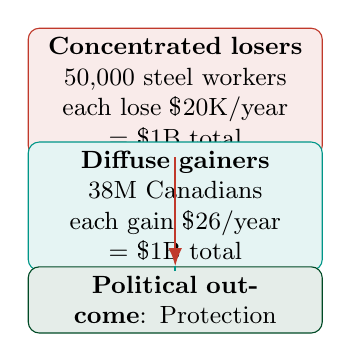
\begin{tikzpicture}[scale=0.85]
\node[draw=AccentRed,fill=AccentRed!10,rounded corners,text width=3.5cm,minimum height=1cm,align=center,font=\small] (losers) at (0,2.5) {\textbf{Concentrated losers}\\50,000 steel workers\\each lose \$20K/year\\= \$1B total};
\node[draw=AccentTeal,fill=AccentTeal!10,rounded corners,text width=3.5cm,minimum height=1cm,align=center,font=\small] (gainers) at (0,0.8) {\textbf{Diffuse gainers}\\38M Canadians\\each gain \$26/year\\= \$1B total};
\node[draw=UNBCDark,fill=UNBCDark!10,rounded corners,text width=3.5cm,minimum height=0.8cm,align=center,font=\small] (pol) at (0,-0.6) {\textbf{Political outcome}: Protection};
\draw[-{Latex},AccentRed,thick] (losers.south) -- (pol.north);
\draw[AccentTeal,thick,dashed] (gainers.south) -- (pol.north);
\end{tikzpicture}
\end{column}
\end{columns}
\end{frame}

\begin{frame}{Stigler's Capture Theory and Rent-Seeking}
\begin{columns}
\begin{column}{0.52\textwidth}
\begin{block}{Stigler's Capture Theory (1971)}
  Regulatory agencies and trade policy institutions tend to be ``captured'' by the industries they regulate. The regulator acts in the interest of the regulated industry rather than the public.
\end{block}
\vspace{0.3em}
\textbf{Why capture happens:}
\begin{itemize}
  \item Industry has deep expertise and provides information to regulators.
  \item Revolving door: regulators often become industry lobbyists.
  \item Industry provides campaign finance; consumers do not.
  \item \textbf{Rent-seeking}: resources spent lobbying for protection are wasteful from a social perspective.
\end{itemize}
\end{column}
\begin{column}{0.45\textwidth}
\begin{canadex}[Supply Management]
  Canada's Dairy Farmers of Ontario and BC Milk Marketing Board control supply quotas and lobby effectively.\\[0.3em]
  \textbf{Annual cost} to Canadian consumers: $\sim$\$700 per household (Conference Board of Canada).\\[0.3em]
  \textbf{Annual gain} to dairy farmers: $\sim$\$600K per farm operation (quota value).\\[0.3em]
  Despite economists' consensus that supply management is inefficient, it persists because the 20,000 dairy farm families have enormous political power.
\end{canadex}
\end{column}
\end{columns}
\end{frame}

\begin{frame}{The Median Voter and Trade Policy}
\begin{columns}
\begin{column}{0.52\textwidth}
\textbf{Median Voter Theorem}: in a two-party system, both parties converge to the position of the median voter.\\[0.3em]
\textbf{Application to trade:}
\begin{itemize}
  \item If the median voter is a \emph{worker} in an import-competing industry, trade protection is the winning policy.
  \item If the median voter benefits from cheaper imports as a consumer, free trade is optimal politically.
  \item The median voter's identity depends on the structure of the economy and how trade distributes gains/losses.
\end{itemize}
\vspace{0.2em}
\textbf{Stokey/Krugman critique}: median voter theory oversimplifies; organised interest groups (steel, auto, dairy) have disproportionate influence beyond vote share.
\end{column}
\begin{column}{0.45\textwidth}
\begin{discuss}
  \textbf{Canada vs.\ US dairy politics:}\\[0.2em]
  Both USMCA and TPP/CPTPP negotiations involved pressure to open Canadian dairy markets. Canada agreed to \emph{small} quota expansions but kept supply management intact.\\[0.3em]
  Why did Canada not simply abolish supply management, given that economists and trade partners favour this? What does the median voter theory predict?
\end{discuss}
\end{column}
\end{columns}
\end{frame}

\begin{frame}{Arguments for Trade Protection: Overview}
\begin{columns}
\begin{column}{0.52\textwidth}
\textbf{Economic arguments (potentially valid):}
\begin{enumerate}
  \item \textbf{Optimal tariff}: large-country ToT gain (Ch.~9).
  \item \textbf{Infant industry}: learning-by-doing + market failures.
  \item \textbf{Strategic trade policy}: oligopolistic rents.
  \item \textbf{Second-best arguments}: other market failures (environmental externalities, labour market distortions).
\end{enumerate}
\vspace{0.3em}
\textbf{Non-economic arguments:}
\begin{enumerate}
  \item National security: strategic industries.
  \item Income distribution: help the poor.
  \item Reciprocity: retaliate against unfair foreign trade practices.
\end{enumerate}
\end{column}
\begin{column}{0.45\textwidth}
\begin{insight}{Economists' Evaluation}
  The optimal tariff and some infant-industry arguments are theoretically valid. But in practice:
  \begin{itemize}\small
    \item Governments cannot easily identify industries that meet the criteria.
    \item Protection creates rent-seeking and tends to become permanent.
    \item Direct subsidies are almost always more efficient than tariffs as a policy instrument.
  \end{itemize}
  \textbf{Verdict}: free trade with targeted adjustment assistance is generally preferable.
\end{insight}
\end{column}
\end{columns}
\end{frame}

\begin{frame}{The Infant Industry Argument: Theory}
\begin{block}{Infant Industry Argument (Hamilton 1791, List 1841)}
  A new industry that has not yet achieved its minimum efficient scale or accumulated necessary learning-by-doing may need temporary protection until it can compete internationally.
\end{block}
\vspace{0.3em}
\begin{columns}
\begin{column}{0.52\textwidth}
\textbf{When the argument is theoretically valid:}
\begin{enumerate}
  \item \textbf{Learning externalities}: firm's learning benefits spill to competitors. Firm cannot appropriate all returns to learning $\Rightarrow$ underinvestment in learning.
  \item \textbf{Capital market failure}: firm cannot borrow against future productivity gains $\Rightarrow$ underinvestment in scale.
\end{enumerate}
\vspace{0.3em}
If these market failures exist, \textbf{temporary} protection creates real welfare gains.
\end{column}
\begin{column}{0.45\textwidth}
\begin{varbox}
\small\textbf{The key test:}\\
For the infant industry argument to be valid, both of these must hold:
\begin{enumerate}\small
  \item The current period cost of protection is outweighed by future efficiency gains.
  \item The market failure (learning externality or capital market failure) prevents the private sector from making these investments itself.
\end{enumerate}
A subsidy directly targeting the market failure is always more efficient than a tariff.
\end{varbox}
\end{column}
\end{columns}
\end{frame}

\begin{frame}{The Infant Industry Argument: Problems in Practice}
\begin{columns}
\begin{column}{0.52\textwidth}
\textbf{Why infant industry protection often fails:}
\begin{enumerate}
  \item \textbf{Government cannot identify winners}: bureaucrats are not better than markets at picking industries with genuine EoS or learning.
  \item \textbf{Temporary becomes permanent}: protected industries lobby to stay protected even after they have matured.
  \item \textbf{Moral hazard}: protection reduces incentives to become competitive.
  \item \textbf{Rent-seeking costs}: protected industry spends resources lobbying to maintain protection.
  \item \textbf{Better instruments}: a direct subsidy achieves the same goal without taxing consumers.
\end{enumerate}
\end{column}
\begin{column}{0.45\textwidth}
\begin{canadex}[Bombardier: Ambiguous Outcome]
  Governments supported Bombardier's C-Series aircraft ($>\$1$B in subsidies).\\[0.3em]
  \textbf{Good news}: A220 is a commercial success under Airbus.\\[0.3em]
  \textbf{Bad news}:
  \begin{itemize}\small
    \item US imposed 300\% tariff (Boeing complaint).
    \item Bombardier had to cede majority to Airbus.
    \item Taxpayers bore losses; Airbus captured the gains.
    \item ``Temporary'' support lasted 20+ years.
  \end{itemize}
  \textbf{Verdict}: the technology was valid but the industrial policy design was flawed.
\end{canadex}
\end{column}
\end{columns}
\end{frame}

\begin{frame}{Strategic Trade Policy}
\begin{block}{Brander-Spencer Model (1985)}
  In an oligopolistic industry with profit shifting, a \textbf{government export subsidy} can shift oligopoly rents from a foreign firm to the domestic firm, potentially raising domestic welfare even net of the subsidy cost.
\end{block}
\vspace{0.3em}
\begin{columns}
\begin{column}{0.52\textwidth}
\textbf{The logic:}
\begin{itemize}
  \item Suppose Boeing (US) and Airbus (EU) are the only producers of commercial aircraft.
  \item EU subsidises Airbus $\Rightarrow$ Airbus commits to higher output.
  \item Boeing reduces output (best response in Cournot competition).
  \item Airbus captures more profit than it costs the EU in subsidies.
\end{itemize}
\vspace{0.2em}
\textbf{Practical problems:}
\begin{itemize}\small
  \item Requires precise knowledge of market structure.
  \item Assumes no retaliation (Boeing also subsidised via US defence).
  \item If both governments subsidise: both waste resources.
\end{itemize}
\end{column}
\begin{column}{0.45\textwidth}
\begin{insight}{Krugman's Assessment (1987)}
  Strategic trade policy is theoretically coherent but \emph{dangerous} in practice:
  \begin{itemize}\small
    \item Governments rarely know the market structure.
    \item Retaliation triggers subsidy wars.
    \item Political process distorts which industries get supported (lobbying $\neq$ strategic value).
  \end{itemize}
  \textbf{Conclusion}: the theoretical case does not translate into a reliable policy guide.
\end{insight}
\end{column}
\end{columns}
\end{frame}

\begin{frame}{The WTO: A Rules-Based Trading System}
\begin{columns}
\begin{column}{0.52\textwidth}
\textbf{History:}
\begin{itemize}
  \item \textbf{GATT (1947)}: General Agreement on Tariffs and Trade. 23 founding members. Eight negotiating rounds reduced average tariffs from $\sim$40\% to $<$4\%.
  \item \textbf{Uruguay Round (1986--94)}: created the \textbf{WTO (1995)}; extended coverage to services (GATS) and intellectual property (TRIPS).
  \item \textbf{WTO today}: 164 members (including China since 2001).
\end{itemize}
\vspace{0.2em}
\textbf{Three core WTO principles:}
\begin{enumerate}
  \item \textbf{Most-Favoured Nation (MFN)}: equal tariff rates to all members.
  \item \textbf{National treatment}: foreign goods treated equally to domestic ones.
  \item \textbf{Bound tariffs}: countries commit to maximum tariff levels.
\end{enumerate}
\end{column}
\begin{column}{0.45\textwidth}
\begin{block}{WTO Dispute Settlement}
  The WTO's Dispute Settlement Body (DSB) provides binding arbitration.\\[0.3em]
  \textbf{Process}: consultation $\to$ panel $\to$ Appellate Body $\to$ implementation.\\[0.3em]
  \textbf{Canada at the WTO}:
  \begin{itemize}\small
    \item \textbf{Won}: US steel safeguard tariffs (2019).
    \item \textbf{Lost}: dairy TRQ allocation.
    \item \textbf{Ongoing}: softwood lumber CVD disputes.
  \end{itemize}
  WTO rules provide leverage for small countries against large ones.
\end{block}
\end{column}
\end{columns}
\end{frame}

\begin{frame}{Regional Trade Agreements: Types and Growth}
\begin{columns}
\begin{column}{0.52\textwidth}
\textbf{Four levels of integration:}
\begin{enumerate}
  \item \textbf{Free Trade Area (FTA)}: zero tariffs among members; each member keeps its own external tariff. Example: \textbf{USMCA/CUSMA} (Canada, US, Mexico).
  \item \textbf{Customs Union (CU)}: FTA + common external tariff. Example: \textbf{European Union}.
  \item \textbf{Common Market (CM)}: CU + free movement of factors (labour and capital). Example: EU Single Market.
  \item \textbf{Economic Union}: CM + policy harmonisation (fiscal, monetary). Example: \textbf{Eurozone}.
\end{enumerate}
\vspace{0.2em}
As of 2023: $>$350 RTAs notified to the WTO.
\end{column}
\begin{column}{0.45\textwidth}
\begin{canadex}[Canada's RTA Portfolio]
  \begin{itemize}\small
    \item \textbf{CUSMA/USMCA} (2020): replaces NAFTA; adds digital trade, stronger IP, labour standards.
    \item \textbf{CPTPP} (2018): 11 Pacific Rim countries. Canada's most ambitious agreement.
    \item \textbf{CETA} (2017): Canada-EU Comprehensive Economic and Trade Agreement. Covers services and investment.
    \item \textbf{Bilateral FTAs}: with South Korea, Chile, Colombia, Honduras, Jordan, Panama, Peru, Ukraine.
  \end{itemize}
  Canada is one of the most RTA-active countries in the world.
\end{canadex}
\end{column}
\end{columns}
\end{frame}

\begin{frame}{Trade Creation vs.\ Trade Diversion: Viner (1950)}
\begin{block}{Two Welfare Effects of RTAs (Viner, 1950)}
\textbf{Trade creation}: RTA induces shift from high-cost domestic production to lower-cost partner imports. Consumers gain; net welfare \textcolor{AccentTeal}{\textbf{rises}}.\\[0.3em]
\textbf{Trade diversion}: RTA shifts imports from low-cost non-member (now facing tariff) to higher-cost member (now tariff-free). Consumers may gain but government loses revenue; net welfare may \textcolor{AccentRed}{\textbf{fall}}.
\end{block}
\vspace{0.3em}
\begin{columns}
\begin{column}{0.52\textwidth}
\textbf{When does creation dominate?}
\begin{itemize}
  \item Partner countries are efficient producers.
  \item Pre-RTA tariffs were high (large creation potential).
  \item External tariff is low (little diversion).
  \item Preference margin between members and non-members is small.
\end{itemize}
\end{column}
\begin{column}{0.45\textwidth}
\begin{canadex}[CUSMA Auto Content Rules]
  CUSMA requires 75\% North American content for autos to qualify for zero tariff.\\[0.3em]
  This is deliberate \textbf{trade diversion}: it diverts auto parts procurement from cheaper Asian suppliers (South Korea, Japan) to more expensive North American ones.\\[0.3em]
  US and Canadian automakers comply to avoid tariffs, even though parts cost more.
\end{canadex}
\end{column}
\end{columns}
\end{frame}

\begin{frame}{Canada-US Softwood Lumber Dispute: A Case Study in Trade Politics}
\begin{columns}
\begin{column}{0.55\textwidth}
\textbf{The dispute (ongoing since 1982):}
\begin{itemize}
  \item US lumber industry alleges Canadian \textbf{stumpage fees} (provincial charges for harvesting Crown timber) are below market value $\Rightarrow$ constitute a subsidy.
  \item US Commerce Dept.\ imposes \textbf{countervailing duties (CVDs)}: 14--24\% in recent rounds.
  \item Canada disputes at WTO and CUSMA dispute panels; wins most rulings.
  \item US generally ignores adverse rulings or finds new grounds for CVDs.
\end{itemize}
\vspace{0.3em}
\textbf{Current status}: $\sim$17\% CVD + anti-dumping duties on Canadian lumber.
\end{column}
\begin{column}{0.42\textwidth}
\begin{adjustbox}{max width=\columnwidth}
\begin{tabular}{lc}
\toprule
\textbf{Group} & \textbf{Effect}\\
\midrule
BC/Alberta mill workers & Lose (\$B/yr)\\
BC forest companies & Lose\\
US homebuilders & Lose (higher costs)\\
US lumber producers & Gain\\
US lumber workers & Gain\\
Canadian federal gov't & Trade dispute costs\\
\bottomrule
\end{tabular}
\end{adjustbox}
\begin{insight}{Lesson}
  Even clear WTO victories don't guarantee compliance. Trade law is enforced imperfectly when domestic politics in the large country resist.
\end{insight}
\end{column}
\end{columns}
\end{frame}

\begin{frame}{Key Takeaways}
\begin{enumerate}
  \item Trade policy is shaped by \textbf{political economy}: concentrated losers lobby effectively; diffuse gainers do not.
  \item \textbf{Capture theory}: regulatory bodies tend to serve industry interests over public welfare.
  \item The \textbf{infant industry argument} is theoretically valid under learning externalities or capital market failure but rarely works well in practice --- subsidies are better.
  \item \textbf{Strategic trade policy} is theoretically coherent but practically dangerous --- invites retaliation and requires precise knowledge governments don't have.
  \item The \textbf{WTO} provides rules-based constraint on protection that has dramatically reduced tariffs globally.
  \item RTAs create \emph{and} divert trade --- net welfare depends on which dominates.
  \item Real trade policy reflects \textbf{political bargaining} as much as economic logic --- Canada's softwood lumber case illustrates how legal victories don't guarantee outcomes.
\end{enumerate}
\end{frame}

\begin{frame}{Synthesis: What Have We Learned in ECON 308?}
\begin{columns}
\begin{column}{0.52\textwidth}
\textbf{The arc of the course:}
\begin{enumerate}\small
  \item \textbf{Ch.~2}: What does trade look like? Gravity model.
  \item \textbf{Ch.~3}: Why trade? Comparative advantage.
  \item \textbf{Ch.~4}: Short-run distributional effects: specific factors.
  \item \textbf{Ch.~5}: Long-run factor endowments: H-O.
  \item \textbf{Ch.~6}: Terms of trade and welfare.
  \item \textbf{Ch.~7}: EoS and intra-industry trade.
  \item \textbf{Ch.~9}: Trade policy instruments and costs.
  \item \textbf{Ch.~10}: Why bad policy persists.
\end{enumerate}
\end{column}
\begin{column}{0.45\textwidth}
\begin{insight}{The Bottom Line}
  Free trade raises aggregate welfare through comparative advantage, scale economies, and variety. But it creates real distributional conflict.\\[0.4em]
  Good trade policy must:
  \begin{enumerate}\small
    \item Facilitate the efficiency gains from trade.
    \item Compensate and adjust those who lose.
    \item Resist politically powerful but economically damaging protection.
    \item Engage multilaterally (WTO, FTAs) to sustain the rules-based system.
  \end{enumerate}
\end{insight}
\end{column}
\end{columns}
\end{frame}

\end{document}
